The beam dimensions and material properties are \(L=0.445\,\mathrm m\), \(h=0.00300\,\mathrm m\), \(b=0.0370\,\mathrm m\), \(E=200\,\mathrm{GPa}\), and \(\rho=7850\,\mathrm{kg/m^3}\). For bending through the thickness, the cross-section and mass properties are
\[
A=bh=111\,\mathrm{mm^2},\quad
m=\rho A=0.871\,\mathrm{kg/m},\quad
I=\frac{bh^3}{12}=8.33\times10^{-11}\,\mathrm{m^4}.
\]
Consequently \(EI=16.7\,\mathrm{N\,m^2}\) and \(a=(EI/m)^{1/4}=2.09\,\mathrm{m/\sqrt{s}}\). The course notes' cantilever equation is \(1+\cos z\cosh z=0\). To calculate the roots without hyperbolic overflow, the MATLAB script solves \(\cos z+\operatorname{sech}z=0\), which is equivalent for real \(z\).

The corresponding wave numbers, frequencies, and shape coefficients follow from
\[
\gamma_j=z_j/L,\quad \omega_j=a^2\gamma_j^2,\quad f_j=\omega_j/(2\pi),\quad
\beta_j=\frac{\cosh z_j+\cos z_j}{\sinh z_j+\sin z_j}.
\]
\begin{center}\small
\begin{tabular}{rrrrrr}
\toprule
$j$ & $z_j$ & $\gamma_j$ (1/m) & $\omega_j$ (rad/s) & $f_j$ (Hz) & $\beta_j$\\
\midrule
1&1.875&4.21&77.6&12.35&0.734\\
2&4.694&10.55&486&77.4&1.018\\
3&7.855&17.7&1362&217&0.999\\
4&10.996&24.7&2669&425&1.000\\
5&14.137&31.8&4412&702&1.000\\
\bottomrule
\end{tabular}
\end{center}
The mode shapes are normalized so their spatial average square is one.
\[
W_j(x)=\frac{\cosh(\gamma_jx)-\cos(\gamma_jx)
-\beta_j[\sinh(\gamma_jx)-\sin(\gamma_jx)]}
{\sqrt{L^{-1}\int_0^L[\cosh(\gamma_jx)-\cos(\gamma_jx)-\beta_j(\sinh(\gamma_jx)-\sin(\gamma_jx))]^2\,dx}}.
\]
Numerical integration checks \(L^{-1}\int_0^LW_jW_k\,dx=\delta_{jk}\). The 1001-point trapezoidal integration gives unit diagonal entries and a largest off-diagonal magnitude of \(8.38\times10^{-6}\). The MATLAB script displays the complete Gram matrix. Higher modes have additional interior nodes and increasing frequencies, consistent with the \(z_j^2\) dependence.
\begin{figure}[H]\centering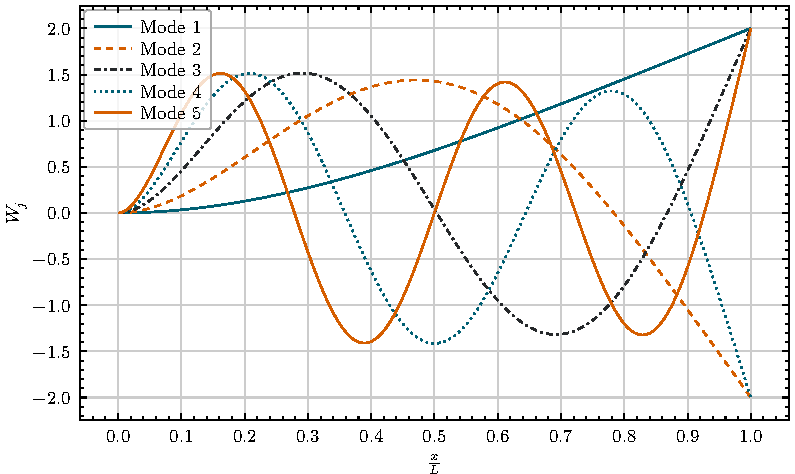
\includegraphics[width=.78\linewidth]{figures/generated/solutions/B3.pdf}\caption{First five normalized cantilever modes.}\end{figure}
\begin{figure}[H]\centering
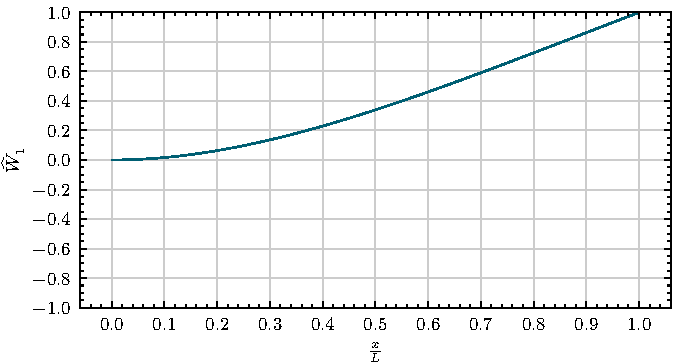
\includegraphics[width=.48\linewidth]{figures/generated/solutions/B3_mode1.pdf}
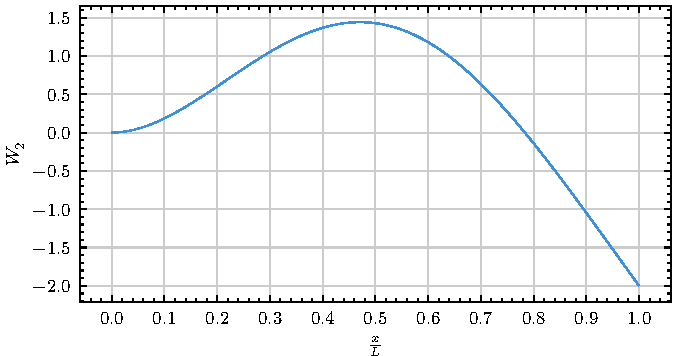
\includegraphics[width=.48\linewidth]{figures/generated/solutions/B3_mode2.pdf}
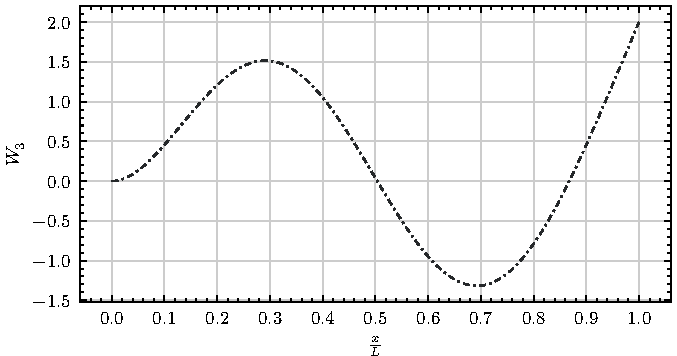
\includegraphics[width=.48\linewidth]{figures/generated/solutions/B3_mode3.pdf}
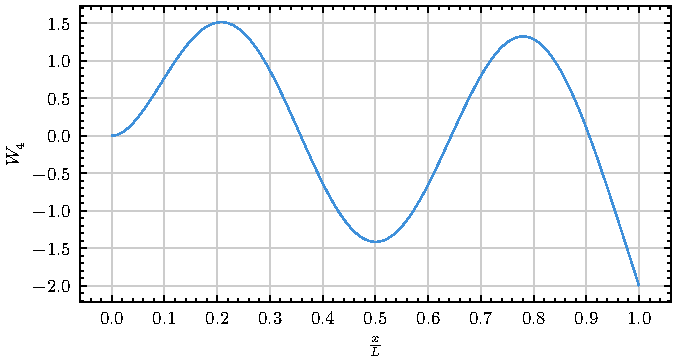
\includegraphics[width=.48\linewidth]{figures/generated/solutions/B3_mode4.pdf}
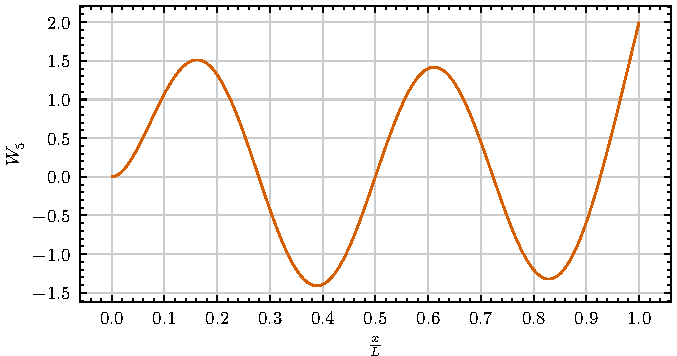
\includegraphics[width=.48\linewidth]{figures/generated/solutions/B3_mode5.pdf}
\caption{Normalized cantilever modes shown individually.}\end{figure}
\matlabcaption{MATLAB calculations and mode shapes for B.3.}
\lstinputlisting[style=hwmatlab]{matlab/B3.m}
